\documentclass{article}

\usepackage[a4paper,landscape,margin=12mm]{geometry}
\usepackage{float}
\usepackage{graphicx}

\pagestyle{empty}
\setlength{\tabcolsep}{3pt}

\begin{document}

\begin{table}[H]
  \centering
  \begin{tabular}{ccc}
    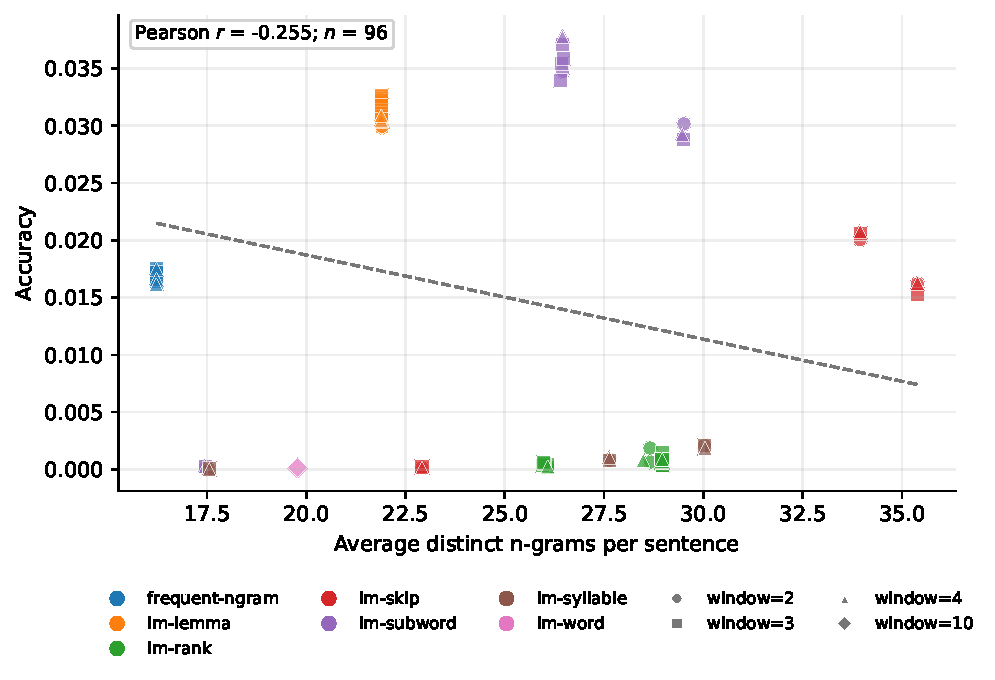
\includegraphics[
      width=0.315\textwidth,
      height=0.36\textheight,
      keepaspectratio
    ]{avg-intrinsic.pdf}
    &
    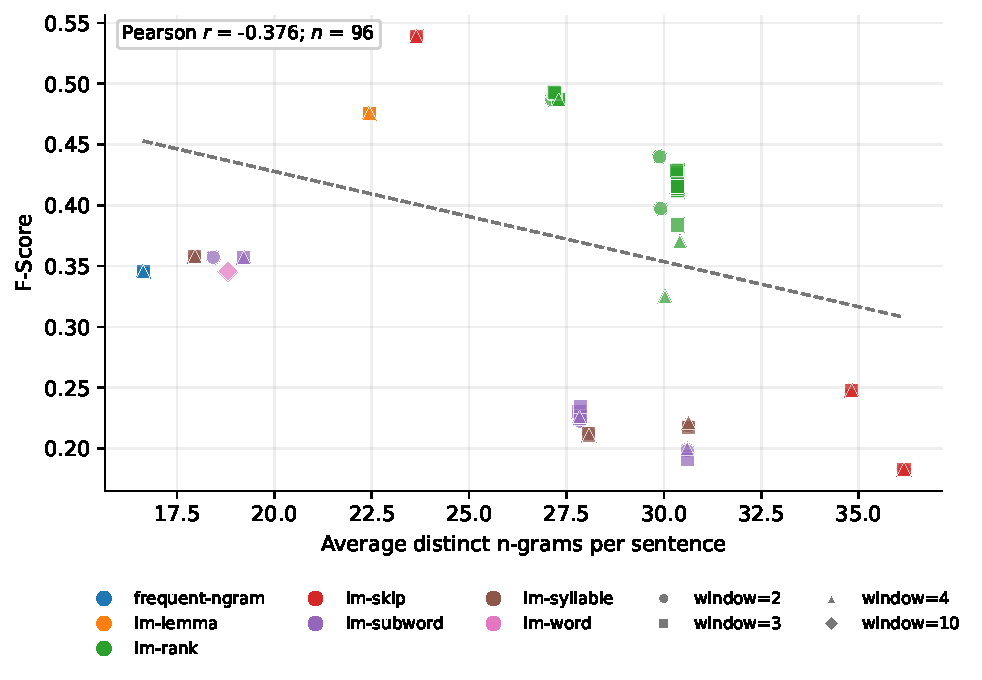
\includegraphics[
      width=0.315\textwidth,
      height=0.36\textheight,
      keepaspectratio
    ]{avg-morphology.pdf}
    &
    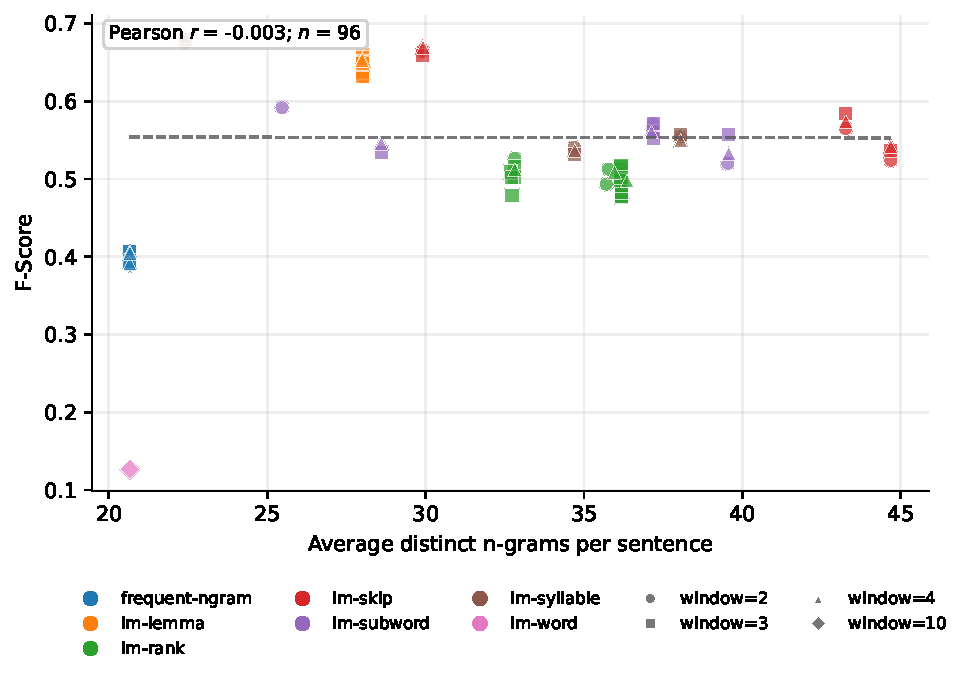
\includegraphics[
      width=0.315\textwidth,
      height=0.36\textheight,
      keepaspectratio
    ]{avg-ner.pdf}
    \\
    Intrinsic & Morphology & NER
    \\
    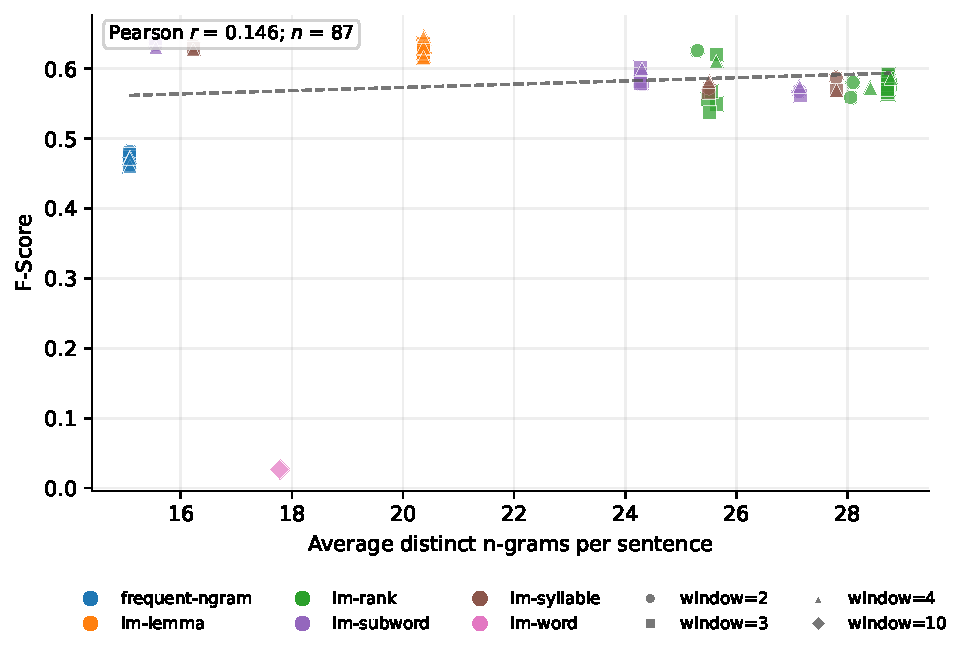
\includegraphics[
      width=0.315\textwidth,
      height=0.36\textheight,
      keepaspectratio
    ]{avg-pos.pdf}
    &
    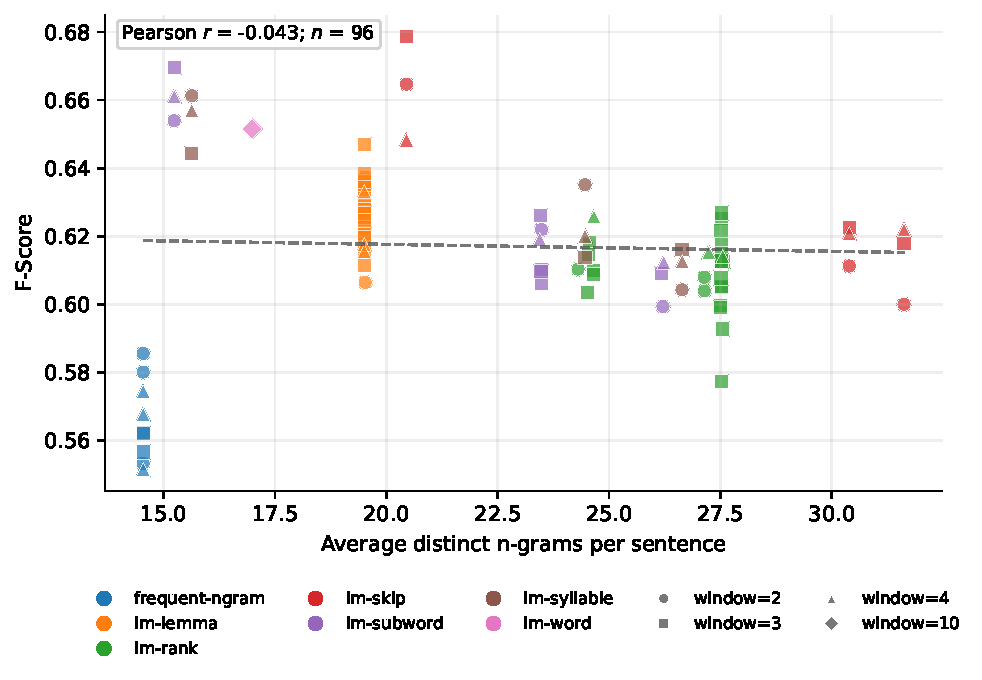
\includegraphics[
      width=0.315\textwidth,
      height=0.36\textheight,
      keepaspectratio
    ]{avg-sentiment.pdf}
    &
    {}
    \\
    POS & Sentiment & {}
  \end{tabular}
  \caption{Average distinct n-grams per sentence and task performance.
  Intrinsic uses Accuracy; Morphology, NER, POS, and Sentiment use
  F-measure.}
  \label{tab:avg}
\end{table}

\end{document}
